
\documentclass[10pt]{beamer}
\usepackage{kotex}

\usepackage{framed}
\usepackage{graphicx}
%https://www.overleaf.com/learn/latex/Inserting_Images

\usepackage{amsmath}
%use dfrac
\usepackage{xcolor}

\usepackage{amsthm}
%\usepackage{tabl}
\usepackage{listings}
\definecolor{mGreen}{rgb}{0,0.6,0}
\definecolor{mGray}{rgb}{0.5,0.5,0.5}
\definecolor{mPurple}{rgb}{0.58,0,0.82}
\definecolor{backgroundColour}{rgb}{0.95,0.95,0.92}
%https://tex.stackexchange.com/questions/348651/c-code-to-add-in-the-document
\lstdefinestyle{CppStyle}{
    backgroundcolor=\color{backgroundColour},   
    commentstyle=\color{mGreen},
    keywordstyle=\color{magenta},
    numberstyle=\tiny\color{mGray},
    stringstyle=\color{mPurple},
    basicstyle=\footnotesize,
    breakatwhitespace=false,         
    breaklines=true,                 
    captionpos=b,                    
    keepspaces=true,                 
    numbers=left,                    
    numbersep=5pt,                  
    showspaces=false,                
    showstringspaces=false,
    showtabs=false,                  
    tabsize=2,
    language=C++
}





\usepackage{url}

\usepackage{etoolbox}
\AtBeginEnvironment{quote}{\singlespacing\small}


\usepackage{thmtools}
\usepackage{xcolor}
\declaretheoremstyle[% spaceabove=6pt,spacebelow=6pt, headfont=\color{MainColorOne}\sffamily\bfseries, notefont=\mdseries, notebraces={[}{]}, bodyfont=\normalfont,
headpunct={},
postheadspace=1em,
%qed=▣,
]{maintheorem}

\declaretheorem[%
name=정의,
style=maintheorem,
numberwithin=section, shaded={%bgcolor=MainColorThree!20,
margin=.5em}]{dfn}
% \begin{dfn}[]
% \end{dfn}

\setbeamertemplate{footline}[frame number]

\usetheme{CambridgeUS}

%\usecolortheme{beaver}


\lstset {language=C++}


\title{template / linker}

\author{EUnS}

\begin{document}

%linker
% #include이해
%template
% TMP맛보기
% 과제 3-2

\begin{frame}{}
    \maketitle
\end{frame}    

\begin{frame}{}
    \tableofcontents
\end{frame}   


\section{compiler}

\begin{frame}
    \begin{figure}[h!]
        \centering
        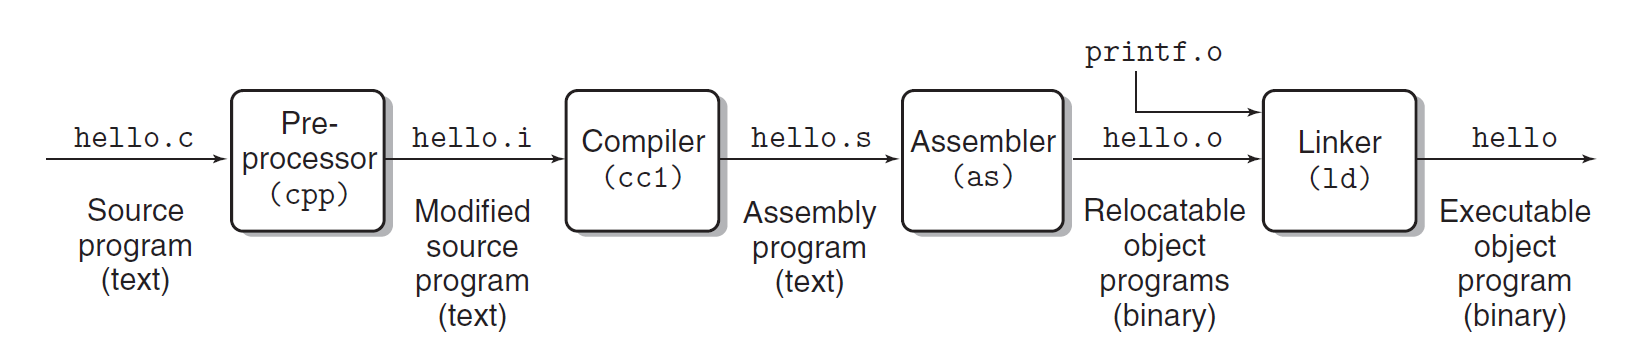
\includegraphics[scale=0.25]{pic/pic1.PNG}
        \caption{컴파일 과정}
    \end{figure}
\end{frame}    

\section{linker}

\begin{frame}
    \begin{itemize}
        \item 서적 : CSAPP (7장 linker)
        \item 아마 시프시간에 배울것.(SNU,kaist..)
        
        \href{http://www.cs.cmu.edu/afs/cs/academic/class/15213-f15/www/schedule.html}{\textcolor{blue}{csapp 강의}}
        
    \end{itemize}
\end{frame}


\begin{frame}{Object File}
    그냥 기계어다.
    \begin{itemize}
        \item Relocatable ob~ : compiler,assembler output
        \item Executable ob~ : linker output
        \item shared ob~ : DLL을 위한 파일 생략
    \end{itemize}
\end{frame}    


\subsection{Relocatable Object Files}

\begin{frame}{ELF}
    x86-linux : object구조로 ELF(Executable and Linkable Format)사용
    \begin{figure}[h!]
        \centering
        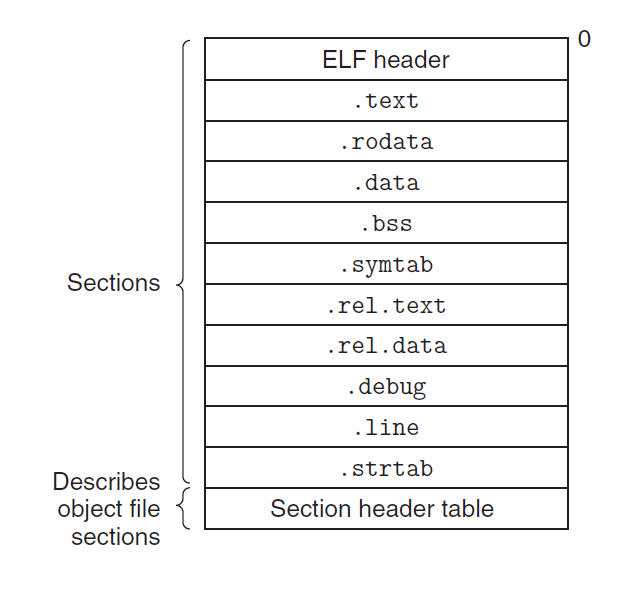
\includegraphics[scale=0.45]{pic/pic2.PNG}
        \caption{Typical ELF relocatable object file.}
    \end{figure}
\end{frame}    

%%%%%%%%%%%%%%%%%%%%%%%%%%%%%%%%%%%%%%%%%%%%%%%%%%%%%%%%%%%%%%%%%%
\begin{frame}{}
    \begin{itemize}
            \item read wirte segment
            \begin{itemize}
                \item .data  :  전역, static 변수
                \item .bss : 초기화 안된 전역 orstatic 변수, 0으로 자동 초기화
            \end{itemize}
            \item read only 
            \begin{itemize}
                \item .text : 머신코드
                \item .rodata : 읽기만 가능한 데이터(ex) jump table)
            \end{itemize}

            \item .symtab : symbol table 
            \item .debug : symbol table for debug
            \item .line : 생략
            \item .strtab : 생략
            
            \item .rel.text 배치해야할 .text
            \item .rel.data 배치해야할 .data 영역

    \end{itemize}
\end{frame}    

\subsection{symbol}


\begin{frame}{symbol}
    \begin{itemize}
        \item Global symbols : 모듈 m에 정의되거나 다른 모듈에 참조될 수 있는 심볼 / 전역변수와 static이아닌 함수
        \item Global symbols : 다른 모듈에 정의된 전역변수 
        /다른곳에 정의된 (extern)전역변수와 static이아닌 함수
        \item Local symbols : static으로 선언된 함수, static 전역변수
    \end{itemize}
\end{frame}

\begin{frame}
    Q : 지역 변수는요?

    A : 런타임에 스택에 쌓습니다.
\end{frame}



\subsection{linker sequence}

\begin{frame}{linker 단계}
    \begin{enumerate}
        \item symbol resolution
        \item Relocation
    \end{enumerate}
\end{frame}    


\begin{frame}{Symbol Resolution}
    \begin{itemize}
        \item strong symbol : 초기화된 전역변수, 함수
        \item weak symbol : 초기화x 전역변수
    \end{itemize}
    
    Rule

    \begin{enumerate}
        \item Multiple strong symbols with the same name are not allowed.
        \item Given a strong symbol and multiple weak symbols with the same name, choose the strong symbol.
        \item Given multiple weak symbols with the same name, choose any of the weak symbols.
    \end{enumerate}
\end{frame}    

\begin{frame}{Relocation}
    \begin{enumerate}
        \item Relocating sections and symbol definitionss :  여러개의 .data section 합친다. 이후 인스트럭션과 전역변수들이 런타임 메모리 주소를 가진다.
        \item Relocating symbol references within sections. :모든 심볼 참조를 수정한다. 이후  
        모든 심볼들이 런타임 메모리 주소를 가진다. 어셈블러가 만든 .rel.data section에 있는 Relocation Entries자료구조를 가지고 수행한다
        \begin{itemize}
            \item R\_X86\_64\_PC32 : 상대주소
            \item R\_X86\_64\_32. : 절대주소
        \end{itemize}
    \end{enumerate}
\end{frame}    

\begin{frame}{Executable Object Files}
    \begin{figure}[h!]
        \centering
        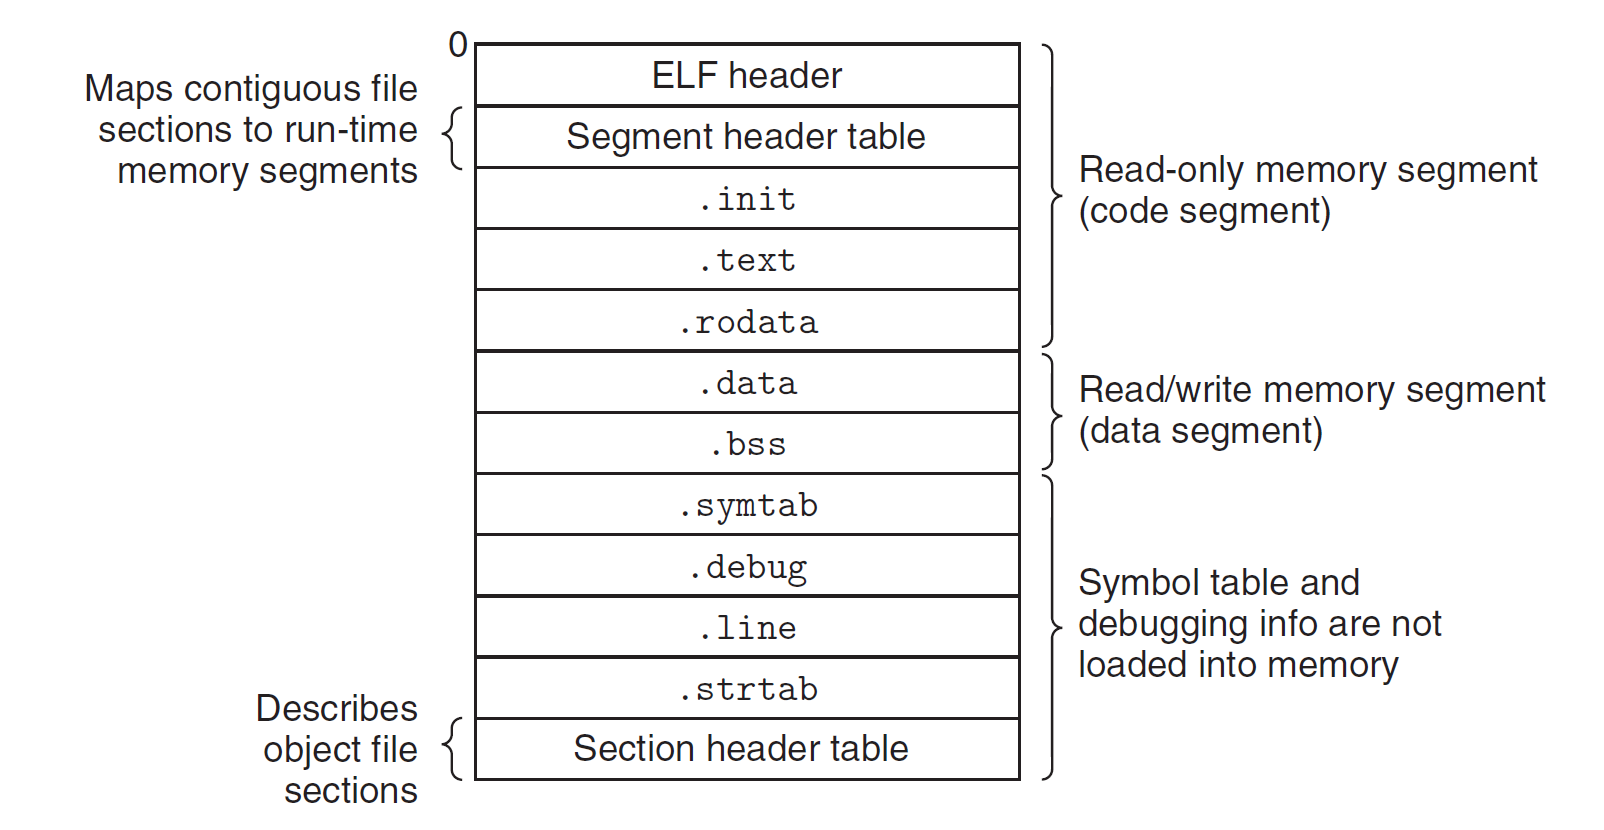
\includegraphics[scale=0.24]{pic/pic3.PNG}
        \caption{Typical ELF executable object file.}
    \end{figure}
\end{frame}    

\begin{frame}{Loading}    
    \begin{figure}[h!]
        \centering
        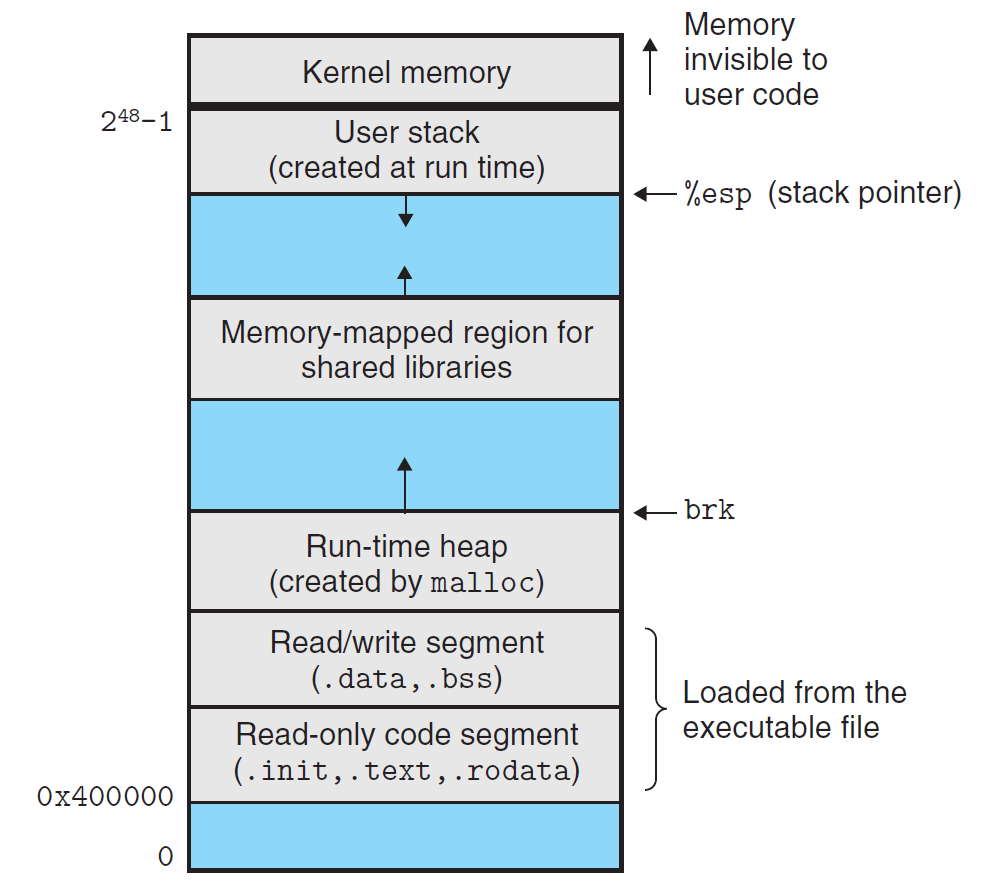
\includegraphics[scale=0.3]{pic/pic4.PNG}
        \caption{\textbf{Linux x86-64 run-time memory image.}}
    \end{figure}
    loading : 실행가능한 목적파일 내의 코드와 데이터를 메모리로 복사하고 첫번째 인스트럭션(엔트리 포인트)으로 점프해서실행하는 과정
\end{frame}    


\section{template}

\begin{frame}[fragile]{template function}
    \begin{itemize}
        \item 타입에 얽메이지 않고 코드를 작성할 수 있게 해줌
        \item container와 기타 라이브러리를 구현한 방법
    \end{itemize}    
    \begin{lstlisting}[style = CppStyle]
        void swap(int &a, int &b)
        void swap(double &a,double &b)
        void swap(name &a, name &b)
        // replace
        template<typename T>
        void swap(T &a ,T& b);
    \end{lstlisting}
\end{frame}    

    
\begin{frame}{template}
    \begin{itemize}
        \item 타입(class) 아무거나 넣어도 가능, 템플릿 인자 여러개 사용가능.
        \item template을 실제로 인자를 넣어서 사용할때 직접 인자를 넣은 실제 코드를 생성함 짜게되는 template 코드는 실제 실행 코드가 아님
        \item 실행 파일크기가 생각보다 커질 수 있음
        \item 템플릿의 링커단계 처리는 컴파일러마다 차이가 있음. (GNU에서는 weak symbol로 처리해서 생성되는 template중 아무거나 택한다.)\href{https://stackoverflow.com/questions/44335046/how-does-the-linker-handle-identical-template-instantiations-across-translation}{\textcolor{blue}{참고}}
    \end{itemize}
\end{frame}    

\begin{frame}[fragile]{}
    \begin{lstlisting}[style = CppStyle]
    template<typename T>
    class name
    {
        T item;
        T function(const T &a,const T &b);
        int a;
    };
    template<typename T>
    T name<T>::function(const T &a,const T &b){;}
    \end{lstlisting}
\end{frame}    

\begin{frame}{template linker error}
    \begin{itemize}
        \item template을 파일 분할을 해보자.
        \item 링커 에러가 뜰것이다.
        \item 왜?
    \end{itemize}
\end{frame}

\begin{frame}{header file}
    \begin{itemize}
        \item 그냥 텍스트파일과 같다.
        \item 선언을 위한것...
        \item 실제 구현은 어느 cpp파일에서...
        \item $\#include$는 \textbf{전처리 지시자}.
        \item $\#include$로 cpp파일에 그대로 붙여넣는다.
    \end{itemize}
\end{frame}






\begin{frame}[fragile]{template specialization}
    \begin{lstlisting}[style = CppStyle]
        #include<iostream>
        using namespace std;
        template<typename T>
        T function(T a)        {
            cout << "Template" << endl;
        }
        template<> // specialization
        char function<char>(char a)        {
            cout << "specialization " << endl;
        }
        char function(char a){
            cout << "overloading" << endl;
        }
        int main(){
            function(1);
            function('s');
        }
    \end{lstlisting}

    \begin{itemize}
        \item 권장되는 방법은 아님 \href{https://wikidocs.net/652}{\textcolor{blue}{참고1}} \href{https://www.codentalks.com/t/topic/2834}{\textcolor{blue}{참고2}}
    \end{itemize}
\end{frame}    


% \begin{frame}{}
% \end{frame}    

% \begin{frame}{}
% \end{frame}    


\section{TMP}

\begin{frame}[fragile]{TMP}
    
    \begin{lstlisting}[style = CppStyle]
    template <int N>
    struct Factorial {
        static const int result = N * Factorial<N - 1>::result;
    };
    template <>
    struct Factorial<1> {
        static const int result = 1;
    };
    cout << Factorial<4>::result; 
    \end{lstlisting}
    
    \begin{itemize}
        \item template의 특성을 이용해서 반복되는 계산을 코드를 생성하여 계산 해놓은다음 그 값을 $O(1)$에 부르는 흑마법
        \item \href{https://libsora.so/posts/friday-the-13th-tmp/}{\textcolor{blue}{이런짓도 가능}}
    \end{itemize}
\end{frame}    


\section{constexpr (c++11)}

\begin{frame}[fragile]{constexpr}
    \href{https://youtu.be/o9FXctFYlnY}{\textcolor{blue}{참고}}
    \begin{itemize}
        \item 변수에 사용할때
        \begin{itemize}
            \item $\#define$ 상수 대체가능
            \item const 상수 완전히 대체가능
            \item 컴파일타임에 상수로 대체
        \end{itemize}
        \item 함수에 사용할때
        \begin{itemize}
            \item 어느부분 TMP 대체가능
            \item 컴파일타임에 계산할수도있고 안할수도있음
        \end{itemize}
    \end{itemize}
    \href{https://www.acmicpc.net/problem/10872}{\textcolor{blue}{boj10872}}
\end{frame} 


%constexpr 코드
\begin{frame}[fragile]{costexpr 활용}
    \begin{lstlisting}[style = CppStyle]
        constexpr int facto(int i){
            int a = 1;
            for (int j = 2 ; j <= i; ++j)	{
                a *= j;
            }
            return a;
        }
        constexpr int Factorial[13] = {
            1,
            facto(1) ,
            facto(2) ,
            facto(3) ,
            facto(4) ,
            facto(5) ,
            facto(6) ,
            facto(7) ,
            facto(8) ,
            facto(9) ,
            facto(10) ,
            facto(11) ,
            facto(12)
        };
    \end{lstlisting}    
\end{frame}

% 과제 3-2

\begin{frame}{과제}
    과제 3-2 : 링크드리스트
\end{frame}    


\end{document}


% \begin{frame}{}
% \end{frame}    
%   \href{https://www.youtube.com/watch?v=OMiEwfmfdng&feature=youtu.be}{\textcolor{blue}
% \begin{frame}[fragile]{}
        
%     \begin{lstlisting}[style = CppStyle]
    
%     \end{lstlisting}

% \end{frame}    


%\lstset {language=C++}
